\documentclass[tikz]{standalone}
\usetikzlibrary{arrows.meta, positioning}

\begin{document}
	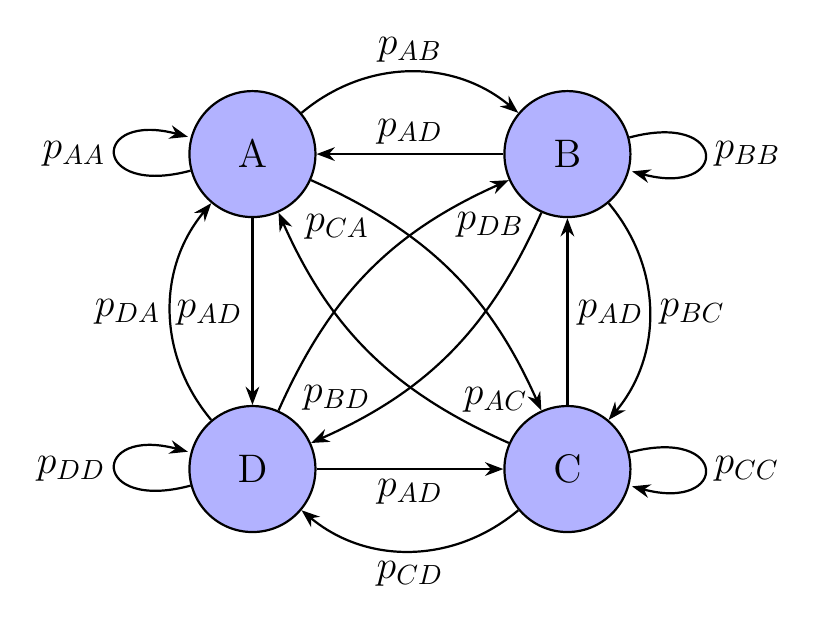
\begin{tikzpicture}[
		state/.style={circle, draw=black, fill=blue!30, minimum size=1.6cm, font=\Large},
		every node/.style={font=\Large},
		>=Stealth,
		thick % Added 'thick' to make all lines thicker by default
		]
		
		% Positions of the nodes
		\node[state] (A) at (0,4) {A};
		\node[state] (B) at (4,4) {B};
		\node[state] (C) at (4,0) {C};
		\node[state] (D) at (0,0) {D};
		
		% Self-loops
		\draw[->] (A) edge[loop left] node[left] {$p_{AA}$} (A);
		\draw[->] (B) edge[loop right] node[right] {$p_{BB}$} (B);
		\draw[->] (C) edge[loop right] node[right] {$p_{CC}$} (C);
		\draw[->] (D) edge[loop left] node[left] {$p_{DD}$} (D);
		
		% Clockwise arrows
		\draw[->] (A) to[bend left=40] node[above] {$p_{AB}$} (B);
		\draw[->] (B) to[bend left=40] node[right] {$p_{BC}$} (C);
		\draw[->] (C) to[bend left=40] node[below] {$p_{CD}$} (D);
		\draw[->] (D) to[bend left=40] node[left] {$p_{DA}$} (A);
		
		% Counterclockwise strait arrows
		\draw[->] (A) to node[mid left] {$p_{AD}$} (D);
		\draw[->] (D) to node[below] {$p_{AD}$} (C);
		\draw[->] (C) to node[mid right] {$p_{AD}$} (B);
		\draw[->] (B) to node[above] {$p_{AD}$} (A);
		
		\draw[->] (C) to[bend left=21]
		node[near end,right, yshift=23pt, xshift = -9pt] {$p_{CA}$} (A);
		\draw[->] (A) to[bend left=21] node[near end, below, yshift=-16pt, xshift=-1.5pt] {$p_{AC}$} (C);
		\draw[->] (D) to[bend left=21] node[near end, right, xshift=5.5pt, yshift=-1pt] {$p_{DB}$} (B);
		
		\draw[->] (B) to[bend left=21] node[near end, left, xshift=-3pt, yshift=1.5pt] {$p_{BD}$} (D);
		
	\end{tikzpicture}
\end{document}
